\documentclass[]{article}
\usepackage{graphicx}
\newcommand*{\affaddr}[1]{#1}
\newcommand*{\affmark}[1][*]{\textsuperscript{#1}}
\usepackage{listings} 
\usepackage{xcolor}
\lstset{
	language=Python,  
	frame=shadowbox, %把代码用带有阴影的框圈起来
	rulesepcolor=\color{red!20!green!20!blue!20},%代码块边框为淡青色
	keywordstyle=\color{blue!90}\bfseries, %代码关键字的颜色为蓝色,粗体
	commentstyle=\color{red!20!green!90}\textit,    % 设置代码注释的颜色
	showstringspaces=false,%不显示代码字符串中间的空格标记
	numbers=left, % 显示行号
	numberstyle=\tiny,    % 行号字体
	stringstyle=\ttfamily, % 代码字符串的特殊格式
	breaklines=true, %对过长的代码自动换行
	extendedchars=false,  %解决代码跨页时,章节标题,页眉等汉字不显示的问题
	texcl=true}
\begin{document}
\title{ENGN4528 Computer Vision – 2021 Computer-Lab 3 (C-Lab3)}

\author{Hongxiang Zhang(u7101924)\\
	\affaddr{\affmark[1]Australian National University}
}


\maketitle

\section{Task-1}
\subsection{}
\begin{lstlisting}
def calibrate(im, XYZ, uv):
	A = np.zeros((2*(len(XYZ)),12))
	for i in range(A.shape[0]): # for each x\_i compute A\_i
		if i%2==0: 
			tmp = np.array(XYZ[i//2])
			A[i,4:8] = (-1*tmp).copy()
			tmp2 = uv[i//2][1]*tmp
			A[i,8:] = tmp2.copy()
		else:
			A[i,:4] = tmp.copy()
			tmp2=(-1*tmp).copy()
			tmp2 = uv[i//2][0]*tmp2
			A[i,8:] = tmp2.copy()
	u,s,v = np.linalg.svd(A) # obtain SVD of A
	C = v[-1]
	C = C.reshape(3,4)
	C = np.linalg.inv(T_norm)@C@S_norm #denormalized
	#     print(C)
	return C
\end{lstlisting}
For calibrate function, there are mainly 4 steps. First, compute A\_i for each point. Second, combine all A\_i matrices to one A matrix. Third, solve the SVD of A to get C. Fourth, denormalized C and reshape.

\subsection{}
Answer: The image I choose is stereo2012a.jpg\\
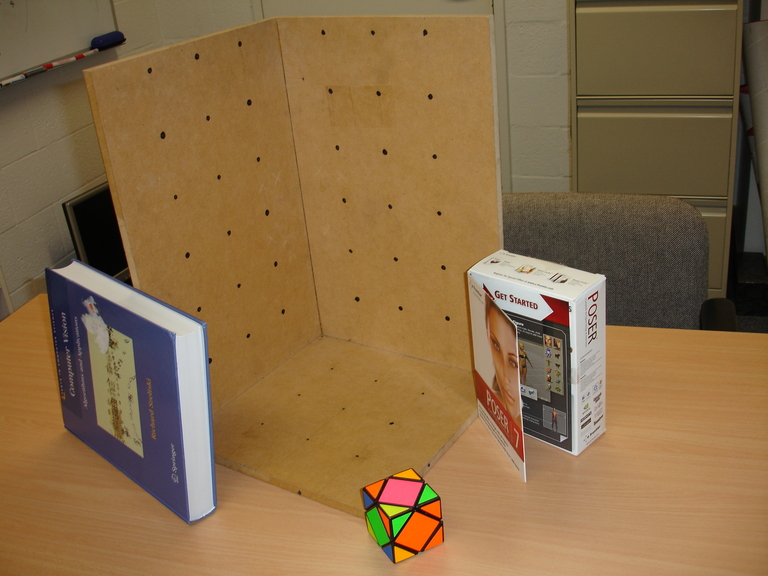
\includegraphics[width=\textwidth]{before.jpg}

\subsection{}
Answer: matrix P: 

[[-1.69926167e+00 , 3.21130575e-01  1.40613179e+00 , -1.03915956e+01]

[-4.35367606e-01 , 1.87301768e+00 -1.08674559e+00 , 1.55109554e+01]

[ 1.32685851e-03 , 1.21078926e-03  2.41171036e-03 , -3.15885150e-01]]

Matrix P is shown above. For the image below, the white cross label indicated the XYZ coordinate I choose, Yellow square label indicated the coordinate which calculates by matrix P.

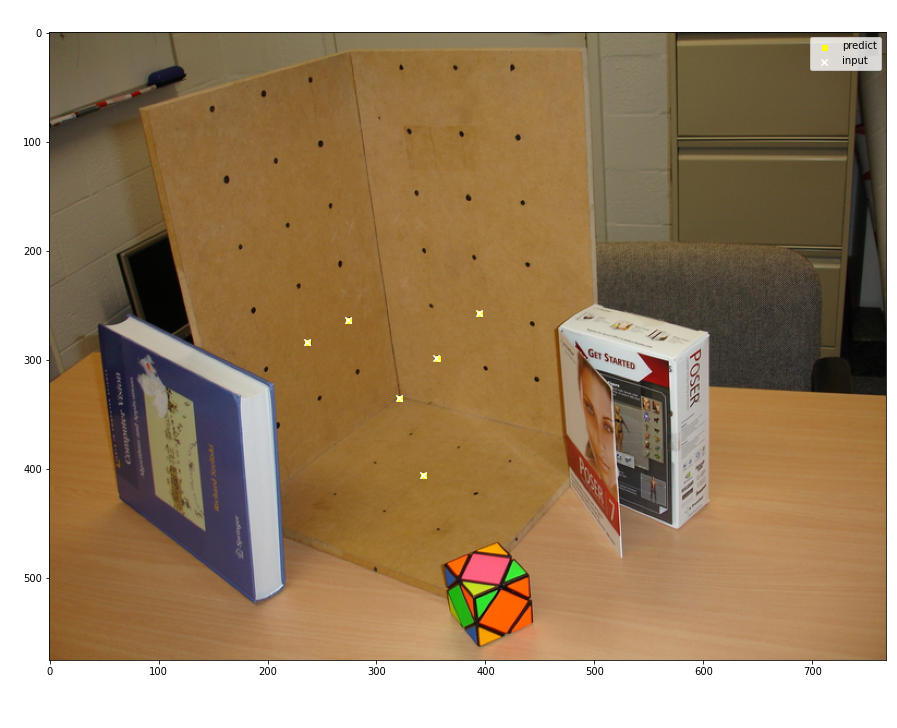
\includegraphics[width=\textwidth]{dlt.png}

\subsection{}
Answer: \\
Using vgg\_KR\_from\_P.py to decompose the P matrix got matrix K,R and t.\\
Matrix K: \\
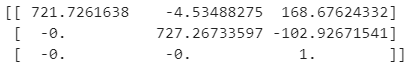
\includegraphics[width=10cm]{k.png}\\
matrix R: \\
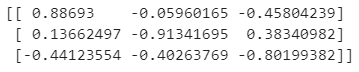
\includegraphics[width=10cm]{r.png}\\
matrix t: \\
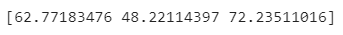
\includegraphics[width=10cm]{t.png}

\subsection{}
Answer: 

There are two directions of focal length, for x axis is k\_00 in matrix K, for y axis is K\_11 in matrix K.\\
Focal length of the camera is fx = 721.7261638, fy = 727.26733597\\

For pitch angle to the X-Z plane, $\theta y$ is the angle we want. The equation is $\theta y = atan2(-R_{31}, \sqrt{r^2_{32} + r^2_{33} } )$ .\\
pitch angle = -26.182739995507493

\subsection{}
uv coordinate after resize:

[[160.5, 167.5], [177.5, 149. ], [137. , 131.5], [171.5, 203. ], [197. , 128.5], [118. , 142. ]]

\subsubsection{a}
Answer: Resized image:\\

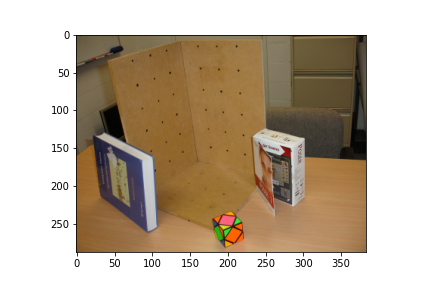
\includegraphics[width=10CM]{shrink.png}\\
matrix K': \\
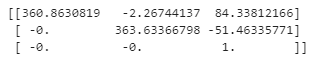
\includegraphics[width=10cm]{k2.png}\\
matrix R': \\
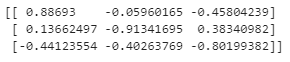
\includegraphics[width=10cm]{r2.png}\\
matrix t': \\
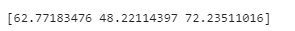
\includegraphics[width=10cm]{t2.png}

\subsubsection{b}
(1)K and K'\\
From the matrix illustrate, K' is 1/2 of K matrix. Matrix K and K' represent the intrinsic parameters matrix which is the camera parameters. what we do is resize the image to 1/2 of the original image, which means one pixel represents more view than the original one. In this case, K\_02, K\_12 is half of the origin K\_02, K\_12, which indicates the cords of principal points. Also, the focal length of x, y-axis, and skew in the y-axis corresponding to K\_00, K\_11, and K\_01 respectively are half of the origin.\\
(2)R and R'\\
From the matrix illustrate, R' did not change. R and R' matrix represent the rotation matrix. The new image just resizes the length of the original image, which means the rotation matrix did not change.\\
(3)t and t'\\
From the matrix illustrate, t' did not change. t and t' represent the traslation. For resized image and origin image, the translation did not change. So the Translation matrix t and t' will not change.

\section{}
\subsection{}
Answer: For homography estimation function, There are mainly 4 steps. First, compute A\_i for each point. Second, combine all A\_i to a matrix A. Third, using SVD to solve A got matrix H. Fourth, denormalized H and reshape.\\
\begin{lstlisting}
	
def homography(u2Trans, v2Trans, uBase, vBase):
	A = np.zeros((2*(len(vbase)),9))
	for i in range(A.shape[0]): # compute A\_i for each point.
		if i%2==0:
			tmp = np.array(uBase[i//2])
			A[i,3:6] = (-1*tmp).copy()
			A[i,5]=-1
			
			tmp2 = u2Trans[i//2][1]*tmp
			A[i,6:9] = tmp2.copy()
			A[i,8] = u2Trans[i//2][1]
		else:
			A[i,:3] = tmp.copy()
			A[i,2] = 1
			
			tmp2=(-1*tmp).copy()
			tmp2 = u2Trans[i//2][0]*tmp2
			A[i,6:9] = tmp2.copy()
			A[i,8] = -1*u2Trans[i//2][0]
	
	u,s,v = np.linalg.svd(A) # SVD
	C = v[-1]
	C = C.reshape(3,3)
	C = np.linalg.inv(T_norm)@C@T_norm # denormalized
	return C
\end{lstlisting}
The image below shows the location of six pairs of selected points.\\
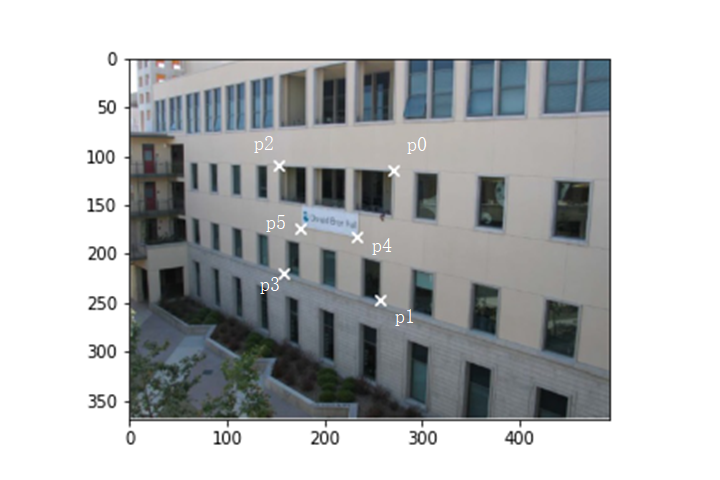
\includegraphics[width=\textwidth]{l.png}\\
In the below image. The white cross label indicate the six selected points, and yellow square label indicate the predicted point after calculate with matrix H.\\
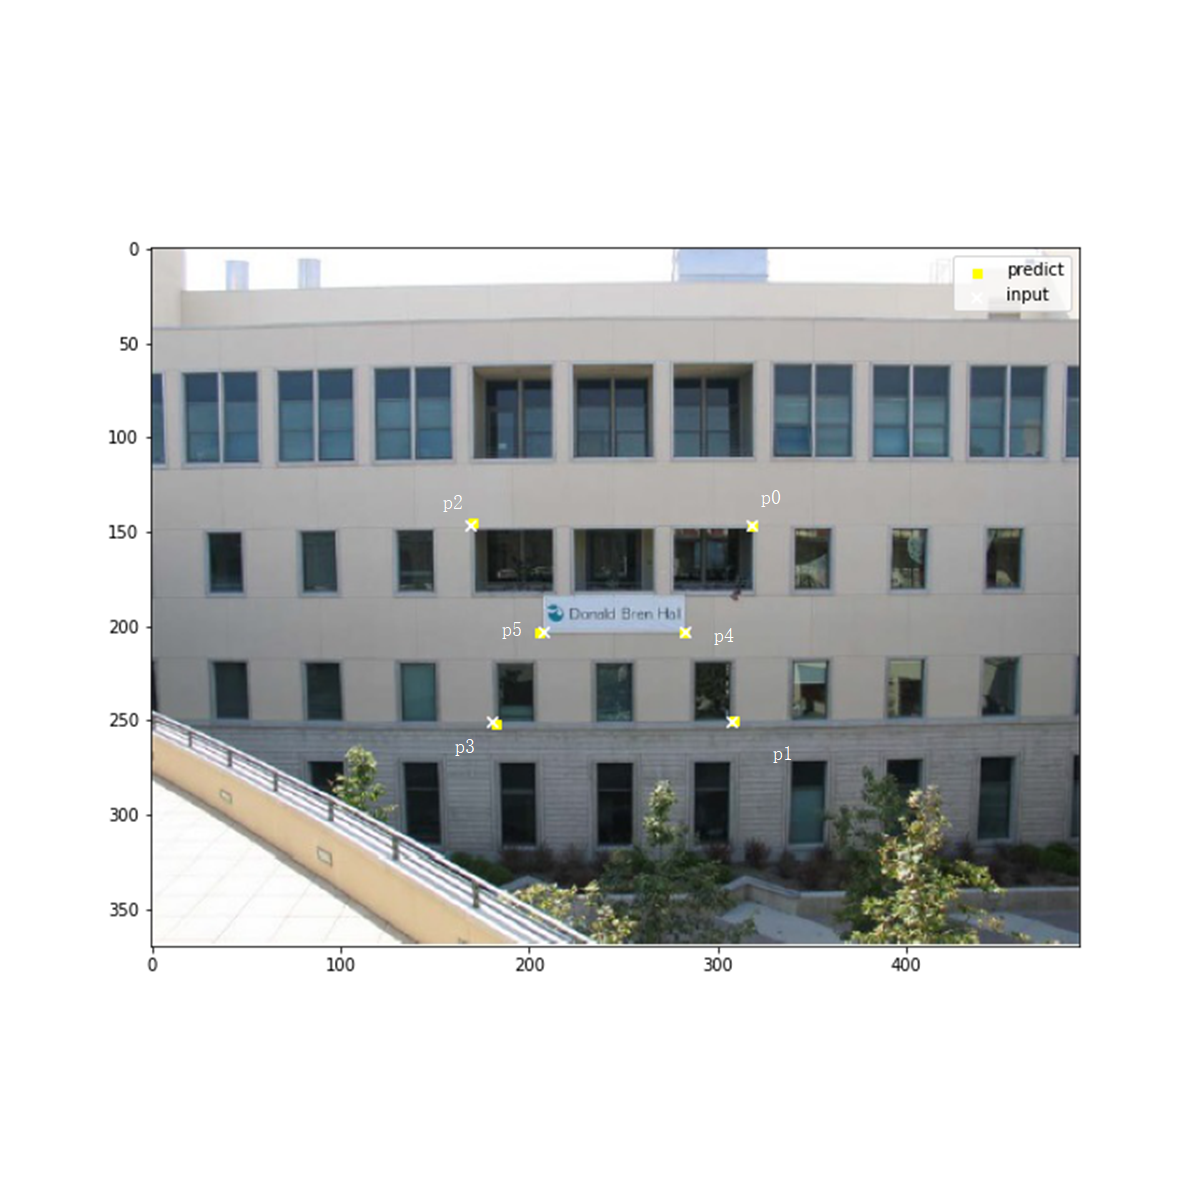
\includegraphics[width=\textwidth]{afterdlt.png}\\

\subsection{}
Answer: Using DLT algorithm to calculate matrix H. H shown below

[[ 6.73269082e-01,  4.92558408e-04, -4.77381102e+01],

[ 1.14736644e-01,  3.06259861e-01, -3.90225861e+00],

[ 8.36792499e-04, -3.85192620e-05,  2.00796437e-01]]

\subsection{}
Answer: Distance for each point in group one is

[0.8552535889510352 , 0.9874512075298797 , 1.5357492316427845 , 1.7922351117891206 , 1.0245671826245484 , 2.275832997005989]\\
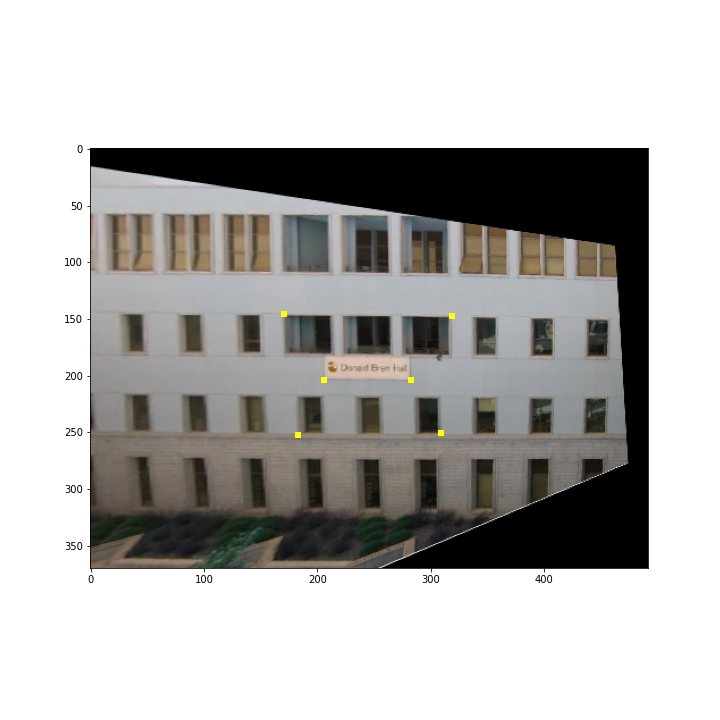
\includegraphics[width=\textwidth]{wraped.png}\\

Distance for each point in group two is

[0.2822897315796688 , 1.1773835682240874 , 0.6670013865970991 , 1.1337963387135694 , 0.04076848450723069 , 0.7024475138312357]

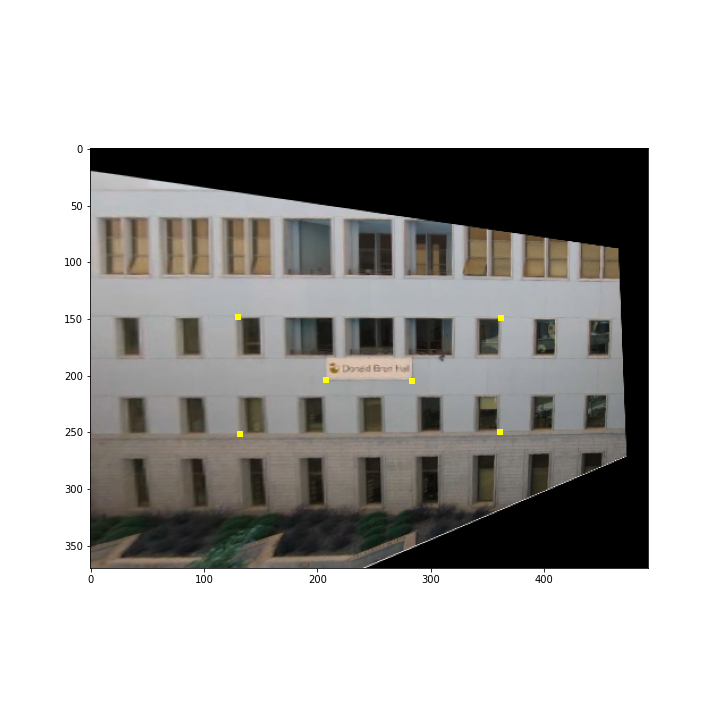
\includegraphics[width=\textwidth]{wraped2.png}\\

As the two images show, the performance of the two images is similar. But the two different matrix show, Those selected points are more sparse have a lower distance than those are dense. In this case, the more sparse selected point has a better performance.

Points 
\end{document}